\documentclass[conference]{IEEEtran}
\IEEEoverridecommandlockouts
% The preceding line is only needed to identify funding in the first footnote. If that is unneeded, please comment it out.
\usepackage{cite}
\usepackage{amsmath,amssymb,amsfonts}
\usepackage{algorithmic}
\usepackage{graphicx}
\usepackage{textcomp}
\usepackage{xcolor}
\def\BibTeX{{\rm B\kern-.05em{\sc i\kern-.025em b}\kern-.08em
    T\kern-.1667em\lower.7ex\hbox{E}\kern-.125emX}}
\begin{document}

\title{Predicting U.S. High School Student Graduation Outcomes Using Two Longitudinal Studies\\
}

\author{\IEEEauthorblockN{1\textsuperscript{st} Josh Wallin}
\IEEEauthorblockA{\textit{Khoury College of Computer Sciences} \\
\textit{Northeastern University}\\
Boston, MA \\
wallin.j@northeastern.edu}
}

\maketitle

\begin{abstract}
High Schools in the United States, as well as state and federal education agencies, have a vested interest in ensuring that
students graduate on time. Often, individual schools and districts have limited resources to support students that are at risk
of failing, and look to identify these students early-on, with the hope of remediating any educational issues before they
lead to a negative outcome. In this project, we focus on a public dataset tracking high school students from 2002 to 2004.
We extract features from these datasets and build a model to predict whether or not a student in 10th grade will later graduate
on-time (i.e., at or before Spring 2004). We apply various techniques to simplify this model and improve its accuracy in the presence
of imbalanced classes. Finally, we attempt to apply the model to data from a similar longitudinal study beginning in 2009.
\end{abstract}

\begin{IEEEkeywords}
machine learning, imbalanced classes, Adaboost, boosting methods
\end{IEEEkeywords}

\section{Introduction}
A variety of players in the American education system have a vested interest in ensuring that students graduate on time. Towards that
end, having the ability to predict student success and target resources before a student fails to graduate is a critical component of risk
management. While detailed longitudinal education data can be difficult to come by, the United States Department of Education has 
collected a small number of detailed studies, capturing demographic, academic, and survey information for students, teachers, and
parents. In this work, we focus on a particular dataset (the Education Longitudinal Study of 2002, ELS:2002)\footnote{https://nces.ed.gov/surveys/els2002/}, along with a related, similar dataset
(the High School Longitudinal Study of 2009, HSLS:2009)\footnote{https://nces.ed.gov/surveys/hsls09/}. \\

Our goal is to develop a predictive model for student graduation, i.e., one that can take as input a student's demographic, academic, and
survey data and predict whether that student will graduate on time or not. The output of this model provides school administrators with an
indicator of whether intervention is needed or not to correct a student's path through school. We test a variety of machine learning algorithms,
including Support Vector Machines (SVM), k-Nearest Neighbors (KNN), Random Forests, and Adaboost. We consider the problem of training a
classifier on our imbalanced dataset and evaluate mitigation techniques to prevent overfitting to the majority class (in this case, students that do
graduate on time) and better recognize members of the minority class (in this case, students that do not graduate on time). We then analyze the
feature importances of our selected model, and simplify it with the goal of maintaining accuracy while reducing model complexity. Finally, we attempt
to apply our training model from the ELS:2002 dataset to similar data given in the HSLS:2009. While we are able to achieve useful accuracy for the 
ELS:2002 dataset, our work does not immediately generalize to the HSLS:2009 dataset and therefore future work will need to consider bridging the gap
between these two. 

\section{Related Work}

For this project, we primarily take inspiration from \cite{b1}. This work focuses on modeling the risk that students across two large school districts
will experience negative educational outcomes, assigning risk scores that can be used by educators in allocating scarce resources. Our problem is simpler 
in the sense that we are concerned solely with binary classification of students as being predicted to graduate on-time or not, and less so with providing a 
risk score.\\

The particular datasets we are considering (ELS:2002 and HSLS:2009) have both been studied in some previous work before. In \cite{b2}, the authors attempt
to predict the final cumulative gpa of high school students base don their performance in tenth grade. This metric is interesting, but not useful in our analysis as
the cumulative gpa of a student is only provided once they have finished high school (i.e., it cannot be used as an input to a model that is meant to predict whether
or not a student will graduate in the first place).\\

The problem of addressing class imbalance has received extensive treatment in the machine learning literature, allowing us to draw on this background in our analysis.
The \texttt{imabalanced-learn} Python toolkit was demonstrated in \cite{b3} and was evaluated by us as a possible technique for reducing dataset problems (thought it 
was not used in the final versions of the models for which performance metrics are given below). The work of \cite{b4} was also consulted, with an eye to determining which
alternative cost strategies might be used with Adaboost to improve our overall model performance. \\

\section{Dataset and Features}

Our primary dataset of concern (initially) is the ELS:2002 dataset provided by the U.S. Department of Education (CITE). This dataset composes a
longitudinal study of high school students, beginning with their sophomore year (10th grade) in 2002. The researchers contacted these students in
follow-up surveys in 2004, 2005, 2006, 2012, and 2013, tracking them through high school, university studies, and their early career. The dataset is
meant to be a nationally representative sample of students in the United States, across demographic characteristics. While the dataset broadly provides
responses at the district and school levels, we focus in this work particularly on student-level and learning environmental characteristics. There are both
restricted-use and public use versions of this dataset; for the sake of this pilot study, we exclusively make use of the public use data files, and have not 
contacted the Department of Education about gaining access to the restricted-use data files. \\

Overall, there is student-level data provided for approximately $\sim16,000$ students, with hundreds of individual features captured. In this work, we consider
only a subset of these features, chosen through the consideration of previous work in modeling a similar problem by (CITE) and consultation with an outside 
education policy expert. The 30 features we specifically consider are as follows:

\begin{center}
\small
\begin{tabular}{| c | p{1.5in} | c |}
\hline
Feature ID & Description & Type\\
\hline
STU\_ID & A student identifier assigned to each student for tracking during the study & Categorical\\
\hline
BYSEX & Sex & Categorical\\
\hline
BYRACE & Race/Ethnicity & Categorical\\
\hline
BYSTLANG & English is the student's first language? & Categorical\\
\hline
BYENGLSE & English self-efficacy score & Continuous\\
\hline
BYHOMLNG & Student's native language & Categorical\\
\hline
BYSTLNG2 & Student's English fluency level & Categorical\\
\hline
BYSES1 & Student's socioeconomic status v1 & Continuous\\
\hline
BYSES2 & Student's socioeconomic status v2 & Continuous\\
\hline
BYG10EP & 10th grade enrollment at student's school & Categorical\\
\hline
BYURBAN & Urbanicity of student's school & Categorical\\
\hline
BYREGION & Region of student's school & Categorical\\
\hline
BYTE15 & Tardiness Rate for student to English & Categorical\\
\hline
BYTM15 & Tardiness Rate for student to Math & Categorical\\
\hline
BYS24E & In-school suspensions received by student & Categorical\\
\hline
BYS24F & Overall suspensions or probation received by student & Categorical\\
\hline
BYGRDRPT & How many grades student has repeated & Categorical\\
\hline
BYLGRRPT & Last grade repeated by student & Categorical\\
\hline
BYIEPFLG & Student has an IEP? & Categorical\\
\hline
BYTXMSTD & Student's math standardized test score & Continuous\\
\hline
BYTXRSTD & Student's reading standardized test score & Continuous\\
\hline
BYPISAME & Student's PISA Math score & Continuous\\
\hline
BYPISARE & Student's PISA Reading score & Continuous\\ 
\hline
BYSTEXP & How far student think's they'll get in their education & Categorical\\
\hline
BYPARASP & How far parent would like student to get in their education & Categorical\\
\hline
BYCONEXP & How successful student expects to be in learning this year & Continuous\\
\hline
BYACTCTL & How much effort and persistence student perceives in self & Continuous\\
\hline
BYHMWRK & How many hours does student spend on homework per week & Continuous\\
\hline
BYS55A & Took or plans to take PSAT? & Categorical\\
\hline
F2HSSTAT & Status of high school completion by 2006 & Categorical\\
\hline
\end{tabular}
\end{center}

This data was provided with normalization already carried out for the continuous features given in the table above,
with the exception of the features BYPISAME, BYPISARE, and BYHMWRK. Selection of data was challenging; the
datasets themselves were so large that a normal data management program (e.g., Microsoft Excel) could not open
them on our computer to provide any useful level of access. As such, a script had to be written to take as input a formatted
specification of relevant features to extract, essentially operating as a crude query to a database. For the sake of training, we
reserved $80\%$ of the dataset ($\sim 13,000$ instances), with the remaining samples preserved for testing the trained models 
($\sim 3,000$ instances)\\

The data was provided in a similar fashion for the HSLS:2009 dataset, though the features themselves frequently differed. As 
such, we had to manually review the second dataset's available features and attempt to derive reasonable surrogates for the
features appearing in the ELS:2002 dataset (e.g., using a combination of HSLS:2009's 'Science self-efficacy score' and 'Math
self-efficacy score' to derive a reasonable comparison to the ELS:2002's 'English self-efficacy score'). It is very likely that this
practice is what led to the incredibly poor accuracy found when applying the 2002 model to the 2009 dataset.\\

\section{Approach}

We divide our approach to this problem into a series of steps and describe each one individually: (1) Model generation, (2) 
Addressing class imbalance, (3) Analyzing Feature Importance, and (4) Model minimization.

\subsection{Model Generation}

Initially, we settled on four possible algorithms for our predictive model: Support Vector Machines (SVM), k-Nearest Neighbors (KNN), 
Random Forest, and Adaboost. This determination was made through a combination of experience in applying these algorithms in class
to supervised learning problems, and consultation with related work such as (CITE). These models were trained and cross-validated using 
standard ranges for possible parameters (e.g., 100 estimators for Random Forest). 5-fold cross validation was additionally performed to determine
whether hyper-parameters could be appropriately tuned, with the goal of achieving the attainable optimal performance for each of the algorithms.\\

We provide a brief explanation of how each of our possible algorithms works below for the reader:

\begin{itemize}
\item \textit{Support Vector Machines (SVM):} SVM attempts to find an $(n-1)$-dimensional hyperplane for data of dimension $n$, with the intent
of maximizing separation between disparate classes of training samples. We used the \texttt{SVC} class provided by \texttt{scikit-learn} for this task.\\
\item \textit{k-Nearest Neighbors (KNN):} A KNN classifier assumes that similar data instances (i.e., instances of the same class) will be found near each other
in $n$-dimensional space. As such, it uses the classes of the $k$-nearest training examples to a given input to decide which class to assign this input.We used the
\texttt{KNeighborsClassifier} in \texttt{scikit-learn} for this task.\\
\item \textit{Random Forest:} The Random Forest classifier is an extension of the weaker Decision Tree classifier which uses a set of several decision trees to vote
on the class of a given input instance. Each decision tree consists of a series of branchings on the various features of the given input, with leaf nodes representing an
assignment of that instance to a particular class. We make use of the \texttt{RandomForestClassifier} in \texttt{scikit-learn} for this task.\\
\item \textit{Adaboost:} Adaboost is a boosting algorithm that makes use of a set of weaker base estimators to compose a stronger classifier. It builds a sequence of 
models (in our case, we use decision trees as the base estimators), where each estimator in the sequence is meant to improve on the misclassified examples seen 
by the previous estimators. We make use of the \texttt{AdaboostClassifier} in \texttt{scikit-learn} for this task.\\
\end{itemize}

\subsection{Addressing Class Imbalance}

As is a common issue in practical machine learning applications, our dataset was imbalanced across the two possible classes: there we nearly eight
times as many students that did graduate on-time as compared to those who did not. Thus, high accuracy on the dataset could be achieved simply by
a classifier that predicted every student was going to graduate on-time. Instead, alternate metrics needed to be considered (such as recall for the negative
examples--students that failed to graduate on time). Additionally, we considered alternative methods for training that attempted to mitigate the issue, such
as oversampling, undersampling, and the use of additional Python machine learning toolkits such as \texttt{imbalanced-learn}. We focused specifically on
preserving overall accuracy on the dataset, while maximizing accuracy on the negative examples. After selecting a useful technique for this (oversampling), 
we experimented with a variety of factors and graphed our results to select a final, most appropriate algorithm for this problem. \\

\subsection{Analyzing Feature Importance}

Upon selecting our most optimal model, we then considered the problem of reducing the number of features composing the model's decision-making. In a 
practical setting, school administrators may not be able to collect all of the data given in the table above, and might instead choose to prioritize collecting 
just a handful of the given metrics. Towards that end, we performed analysis of the importance of the features composing our optimal model. We used multiple 
metrics for this task, taking into account criticisms provided in both the \texttt{scikit-learn} documentation and additional research. This analysis directly contributed
to the following step in our approach.\\

\subsection{Model Minimization}

After performing our feature importance analysis, we then attempted to reduce the size of our model by limiting the number of features used in its training. We limited
the number of included features given in the table above for any given instance by applying two different feature importance metrics to the already trained larger classifier.
We then analyzed the performance of our models according to the criteria previously established (accuracy on the negative testing examples and overall accuracy on the
testing examples) before selecting the most optimal of these two. We then compared this model to our previous, larger classifier, to determine if there was a significant drop
in accuracy after performing this minimization.\\

\section{Experiments and Results}

\subsection{Performance of Algorithms}

For each of our models, we captured both the overall accuracy as well as the accuracy specifically on the negative class (i.e., recall with respect to the negative class). Our results
were as follows:\\

\begin{tabular}{| c | c | c |}
\hline
Algorithm & Overall Accuracy & Negative Accuracy\\
\hline
SVM & 0.84 & 0.0\\
KNN & 0.81 & 0.22 \\
Random Forest & 0.85 & 0.31\\
Adaboost & 0.85 & 0.26\\
\hline
\end{tabular}
$\;$\\
As can be seen by comparing the overall and negative accuracy, it is clear that the class imbalance has had an impact on the training of these models.No particular model stands out amongst the others, though SVM clearly has some issues in recognizing any of the students in the negative class. This suggests perhaps that the higher dimensional feature space is sufficiently complicated as to make separability by the algorithm impossible. The problem as previously framed, however, is to assist schools in detecting which students are not on track to graduate on-time, so they may be targeted for early intervention. As such, it is critical that any proposed algorithm be capable of performing well with respect to finding which students are struggling (i.e., correctly finding members of the negative class).\\

\subsection{Minimizing the Effects of Class Imbalance}

We attempted a variety of off-the-shelf methods to alleviate the class imbalance of this problem (e.g., through the \texttt{imbalanced-learn} toolkit). For this section, we just focus on the final technique that we selected for training our model: undersampling. Undersampling in the case of class imbalance involves randomly selecting members of the majority (more frequently appearing) class and removing them from the training dataset. This serves to create greater parity between the two classes in the training data. In the end, we decided to implement undersampling ourselves rather than using a more advanced algorithm, after preliminary tests did not demonstrate a significant improvement in performance. Below, we graphed the performance of our various models for a variety of possible ``downscaling factors", which denote the amount of data from the majority class that were withheld when training each model type. \\

\begin{center}
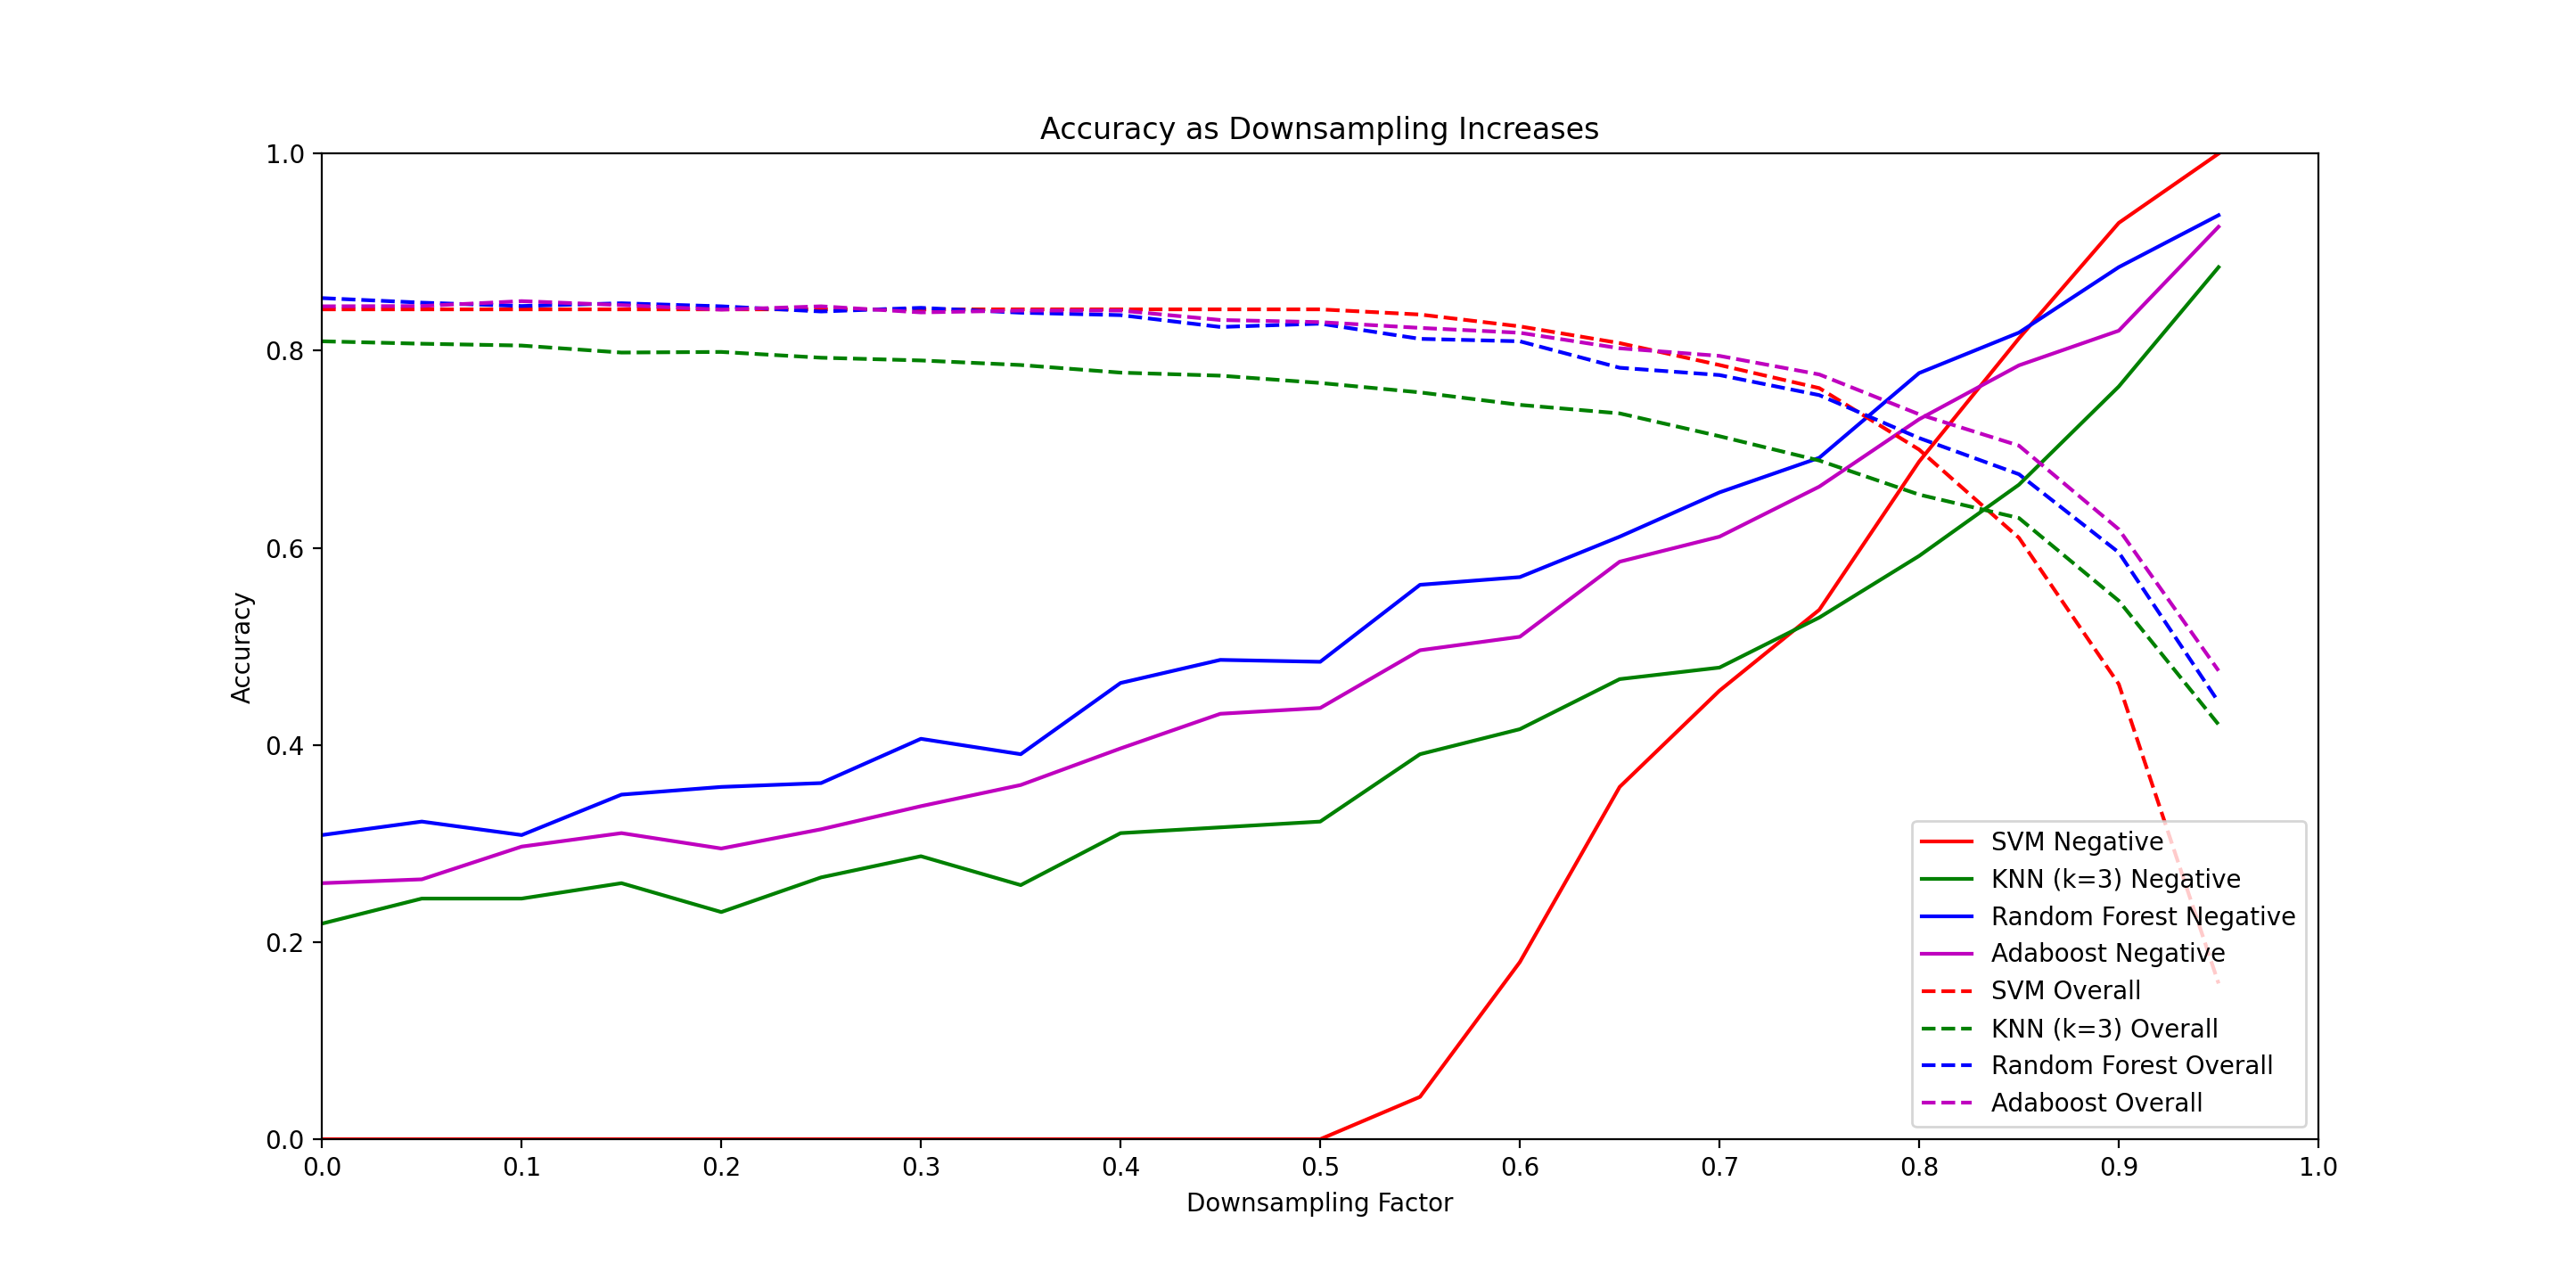
\includegraphics[scale=0.25]{Accuracy_as_Downsampling_Increases.png}
\end{center}

For each model, the ``Negative" (solid) line indicates the accuracy of the model specifically on the negative class examples, while the dashed line indicates overall accuracy on the test dataset. As can be seen, accuracy on the negative examples improves dramatically as the downsampling factor is increased, while accuracy on the overall dataset suffers. For the sake of our use case, we decided that our criteria for the best model was the one that had the highest intersected accuracy between these two lines (i.e., the intersection point between the respective dashed and solid lines with the greatest y-value). This model was found to be the one using the Adaboost algorithm, for a downsampling of $80\%$ (i.e., a reduction in the number of majority-class training examples by $80\%$). This downsampling produces an approximate ratio of $1.1:1$ for positive to negative examples. \\

\subsection{Performing Feature Importance Analysis}

After selecting the Adaboost model as the best-performing according to our criteria, we then began the process of determining which features most contributed to any particular classification decision. Within \texttt{scikit-learn}, the feature importances are captured as an attribute of the model. These importances are also known as Gini importances, and 
are computed as the total reduction of the classifier's accuracy brought by the feature. The higher the value given by this metric, the more important the particular feature is.\\

As noted in the \texttt{scikit-learn} documentation, however, this importance metric can be negatively impacted by features that have a high cardinality. Given the variance in cardinality of the features used in our dataset, we also calculated the permutation importance of the features in our Adaboost model using the built-in \texttt{scikit-learn} function. This metric is meant to capture the effect on the accuracy of our classifier that is brought about by randomly permuting the elements in a particular column (feature) of our dataset. Intuitively, a feature is more important if changing its value results in a significant change in the accuracy of our model. This procedure was performed $10$ times, with the mean importance assigned to each feature being reported. We produce a bar graph of the results of each of these two metrics for each feature below, where the number of a feature corresponds to its row in the table given above (starting from 0). \\

\begin{center}
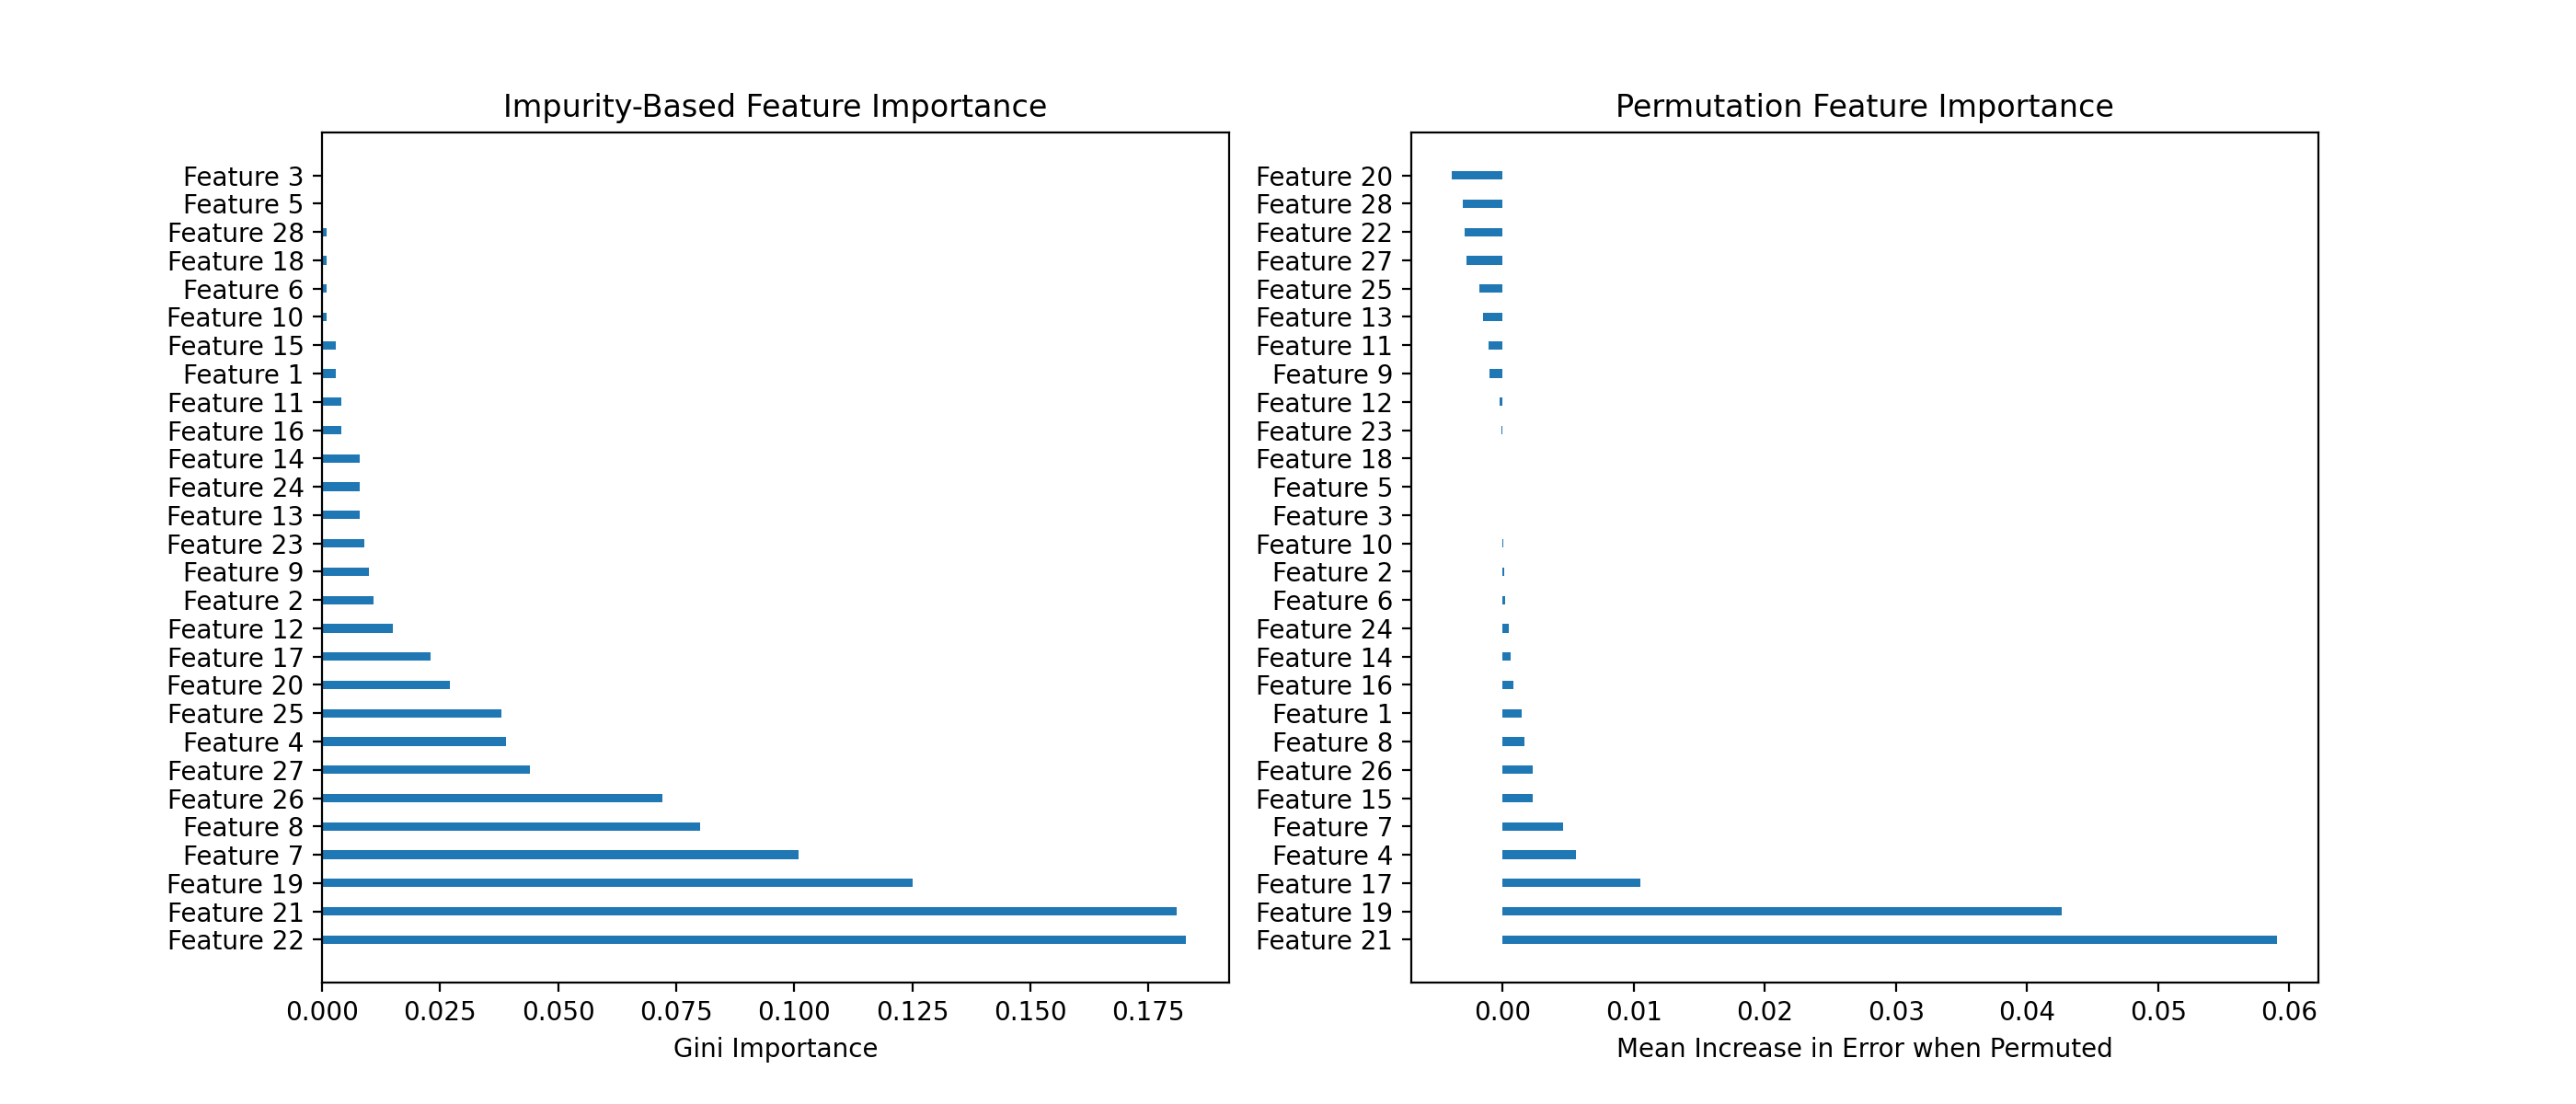
\includegraphics[scale=0.28]{Feature_Importances.png}
\end{center}

As can be seen by the variance in feature importance given by both metrics, some features dominate the classification task significantly more than others. Consultation with an education policy expert confirms that previous research has supported the importance of some of these factors (e.g., socio-economic status), while others were surprising given other research (e.g., number of hours per week spent on homework).\\

\subsection{Model Minimization}

In the interest of minimizing the overall size of the model, we selected the top 10 most important features given by each of the metrics above and evaluated their accuracy across 50 train-test runs. The highest accuracy tests are provided below for each scheme:\\

\begin{tabular}{| c | c | c |}
\hline
Metric & Overall & Negative Class\\
Impurity-Based & 0.69 & 0.72\\
Permutation-Based & 0.71 & 0.73\\
\hline
\end{tabular}

$\;$\\
As can be seen, neither model particularly out-performed the other with respect to our established metrics. Both models performed comparably to the larger (fully featured) model, and were thus considered sufficient for future tests.\\

\subsection{Generalization of Model}

While significant future work must be applied to this problem, we did attempt to extract the relevant features from the HSLS:2009 dataset and apply the ELS:2002 model to them. While a full, experimental approach to this problem could not be completed during the course of this project, an attempt was made to adapt the relevant features from the former dataset to the latter model (i.e., to derive the relevant features from this dataset so the ELS:2002 model could be used). Initial tests indicate abysmal accuracy ($\sim1\%$). This result likely indicates that the methods used for adapting the data were not sufficient, and so this task should fall into the realm of future work.\\

\section{Conclusion and Future Work}

In this project, we evaluated the success of performing modeling and analysis of the ELS:2002 dataset from the Department of Education, with a specific focus on optimizing the model in the presence of imbalanced classes and with the intent of maximizing its classificatory capabilities with respect to students that are unlikely to graduate high school on-time. We performed analysis of a variety of modeling algorithms with various parameters, and determined that an Adaboost classifier with downsampling of the majority class in the training data was the best way to train the classifier.\\

While this work was useful for the 2002 dataset, it failed to generalize to the 2009 dataset. Future work should primarily focus on finding useful strategies to adapt the data provided in the HSLS:2009 dataset to those provided in the ELS:2002 dataset, to determine how the 2002 model we trained above can appropriately be applied. This will require further consultation with professionals in this field.

\section*{Contributions}
This work was performed by Josh Wallin, with education policy questions answered by Terra Wallin. All code and results files can be found at 
\begin{verbatim*}
https://github.com/wallinjoshua/
CY6720_Final_Project.git
\end{verbatim*}.\\

\begin{thebibliography}{00}
\bibitem{b1} Himabindu Lakkaraju, Everaldo Aguiar, Carl Shan, David Miller, Nasir Bhanpuri, Rayid Ghani, and Kecia L.
Addison. 2015. A Machine Learning Framework to Identify Students at Risk of Adverse Academic Outcomes. \textit{In
Proceedings of the 21th ACM SIGKDD International Conference on Knowledge Discovery and Data Mining (KDD '15).}
Association for Computing Machinery, New York, NY, USA, 1909–1918. DOI:https://doi.org/10.1145/2783258.2788620
\bibitem{b2} Kennedy, et al. 2020. Understanding Student Success. https://github.com/ybacoder/project-3.
\bibitem{b3} Guillaume Lemaitre and Fernando Nogueira and Christos K. Aridas. 2016. Imbalanced-learn: A Python Toolbox to Tackle the Curse of Imbalanced Datasets in Machine Learning. \textit{Journal of Machine Learning Research }. 18. pp.1-5. 
\bibitem{b4} Nikolaou, N., Edakunni, N., Kull, M. et al. Cost-sensitive boosting algorithms: Do we really need them?. Mach Learn 104, 359–384 (2016). https://doi.org/10.1007/s10994-016-5572-x
\end{thebibliography}
\vspace{12pt}

\end{document}
